\documentclass[../Main.tex]{subfiles}

\begin{document}

\section*{Descripción de los datos}

Los datos para este proyecto son entregados por la Agencial Espacial Europea en formato CSV (2 GBytes) para los últimos cuatro años marcianos. Cada año marciano corresponde a 687 días terrestes.
\newline \par
Los tres primeros años están destinados para entrenamiento de un sistema predictivo y tienen información sobre el consumo eléctrico del sistema termal. El cuarto año no tiene información sobre el consumo eléctrico del sistema termal.
\subsection*{Contextos}
Los datos se encuentran separados según el tipo (o contexto) de información que contienen. Así, existen cinco tipos de contextos de datos:
\begin{itemize}
    \item SAAF: Solar Aspect Angles
    \item DMOP: Detailed Mission Operations Plan
    \item FTL: Flight dynamics Timeline
    \item EVTF: Other Events
    \item LTDATA: Long Term Data such as Sun-Mars distance
\end{itemize}

Cada uno de los tipos de contexto tienen diversas categorías (o columnas).
\subsubsection*{SAAF: Aspectos solares}
Los ángulos entregan información sobre la incidencia de los rayos del sol sobre los paneles solares. Los ángulos se miden con respecto a la línea Sol-MEX.
\subsubsection*{DMOP: Detalles de la planificación de operación}
Los archivos DMOP entregan información sobre los comandos que han sido activados en cada sistema. Cada comando incluye el nombre del sistema y el nombre del comando. Debido a la cantidad de comandos, estos no se explican, sin embargo cada uno tiene distintos efectos sobre la temperatura en los distintos subsistemas, y por esto afectando el sistema termal. En estos comandos se encuentran el encendio y apagado del sistema de telecomunicaciones y de los instrumentos científicos.
\subsubsection*{FTL: Eventos de la trayectoria de la nave}
Los eventos listados en estos datos pueden impactar el comportamiento del satélite ya que pueden afectar los ángulos de incidencia, así como también tener relación con el encendido o apagado de algunos instrumentos.
\subsubsection*{EVTF: Otros eventos}
Este set de datos contiene varios eventos. Contiene información sobre eventos del FTL y la complementa con información sobre otros eventos, como por ejemplo eclipses y sus fases (Penumbra y umbra).
\subsubsection*{LTDATA: Información de periodos extendidos}
Incluye información sobre la distancia entre el Sol y Marte, distancia a la Tierra, duración de los eclipses, etc.

\subsection*{Consumo energético}
En estos sets se incluye información sobre la corriente medida en los 33 circuitos eléctricos de la nave. Cada medición se realiza cada 30 o 60 segundos. 
\newline \par 
El objetivo de la competencia es predecir el consumo promedio por hora del satélite, por lo que la información sobre el consumo eléctrico solo está presente en los datos de entrenamiento.

\section{Exploración inicial}
Como se mencionó anteriormente, el objetivo de la competencia es predecir el consumo energético de los sistemas termicos de la nave a partir de los otros datos que se tienen. La exploración inicial de los datos consistirá en analizar los datos de consumo energético y relacionarlos con los otros datos de estado de los sistemas, incidencia solar y posición del satélite.
\newline \par 
Luego de importar los datos en R, lo primero que llama la atención es la cantidad de datos. El conjunto de datos que intuitivamente contiene más información es el de los datos del consumo energético. Éstos se muestrean cada 30 o 60 segundos. Para el primer año existen 1.830.121 regitros.

\begin{center}
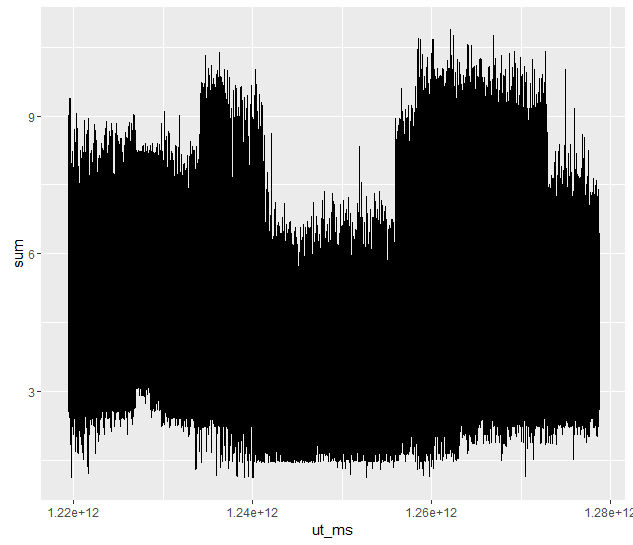
\includegraphics[width=3in]{Assets/power1SumAll.png}
\end{center}

Al graficar este conjunto de datos se puede apreciar que existen niveles de comportamiento. Por la cantidad de datos que existen, el gráfico se aprecia como una mancha continua con secciones de rangos. Debido a esto se procede a graficar en rangos más pequeños.

\begin{center}
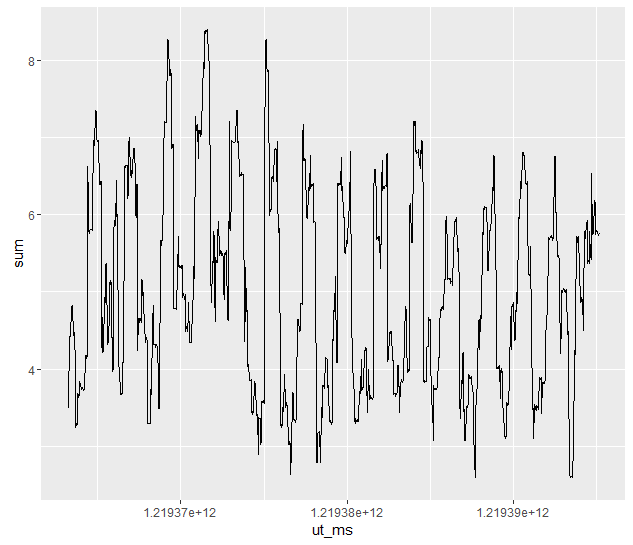
\includegraphics[width=2in]{Assets/power1Sum1k.png}
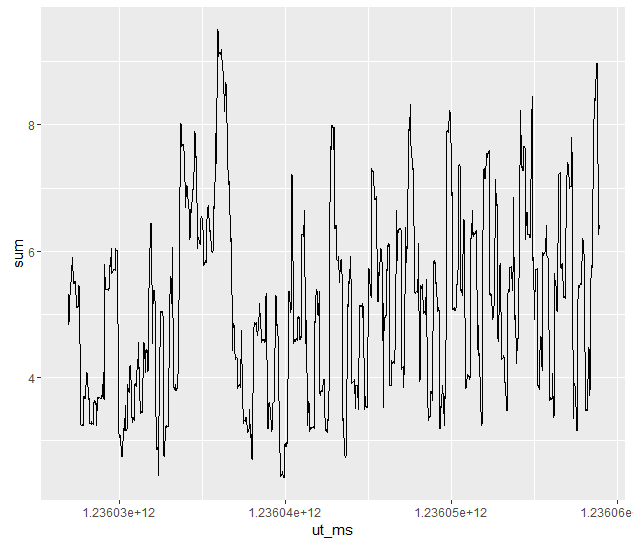
\includegraphics[width=2in]{Assets/power1Sum5hk1k.png}
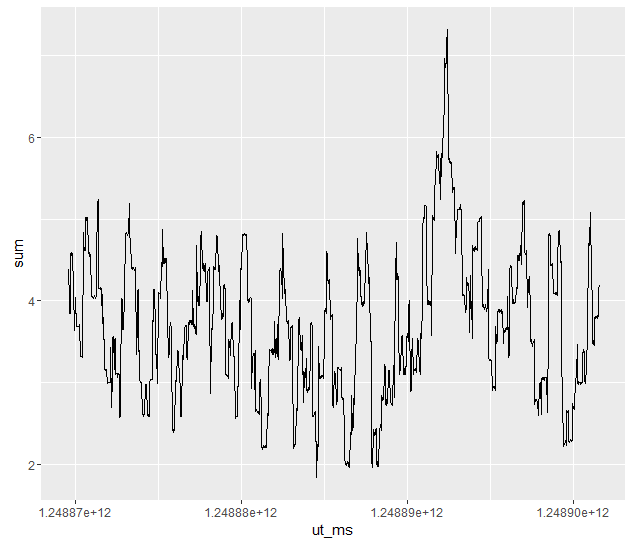
\includegraphics[width=2in]{Assets/power1Sum9hk1k.png}
\end{center}

Al graficar en rangos de mil datos, se puede apreciar mejor el comportamiento de los datos a lo largo del tiempo. Cabe notar que los datos anteriores corresponden a la suma total de los datos de consumo. Se intuye que al revisar los datos del consumo, se encontrará evidencia de la existencia de clusters de circuitos, es decir, de los 33 circuitos, deben haber varios grupos, divididos entre refrigeración/calefacción y entre los distintos sensores y secciones del satélite.
\newline \par 
Una parte importante del trabajo consistirá en encontrar estos clusters. Una vez agrupados los datos se podrá proceder a relacionarlos con comandos enviados remotamente para el encendido y apagado de interfaces y así determinar una relación directa entre estos. 
\newline \par 
De la misma forma, de la primera observación de los datos, se prevee que pueda existir una relación con la distancia con el sol, similar a las estaciones del año. Esto podría influir en el consumo energético de forma significativa.
\newline \par 
Con respecto a los otros set de datos, se considera importante el ángulo de incidencia solar. Al graficar el total de datos de ángulos de incidencia sobre el tiempo, se puede apreciar que el comportamiento es aparentemente similar a una sinusoide. Al compararlo con gráficas de ángulos de incidencia en la Tierra, se infiere que el comportamiento debería ser, efectivamente, una sinusoide. 
\begin{center}
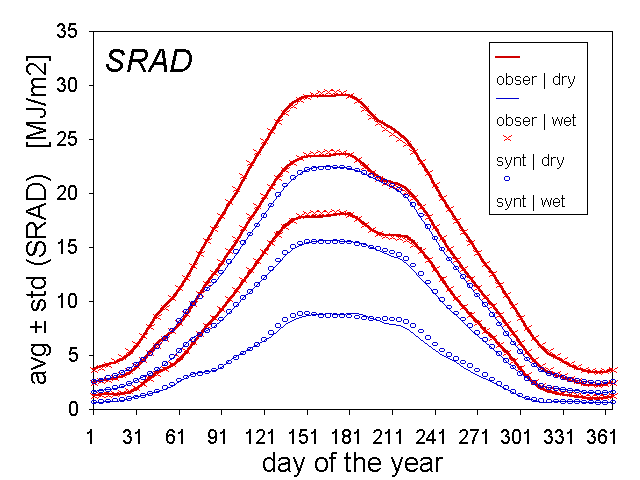
\includegraphics[width=2in]{Assets/srad_sm.png}
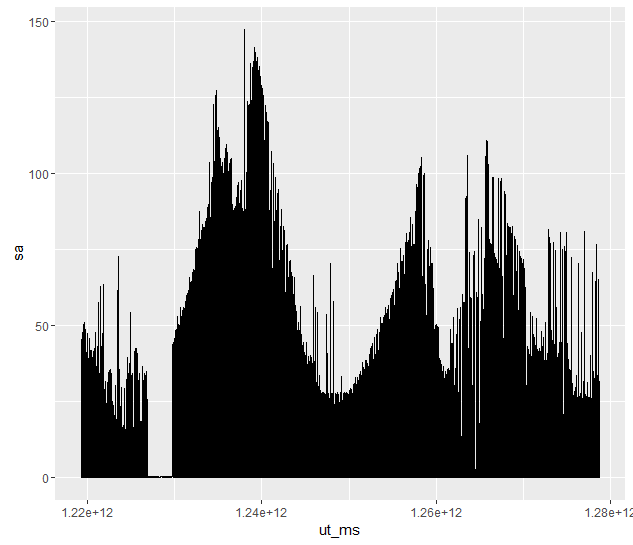
\includegraphics[width=2in]{Assets/saaf1saAll.png}
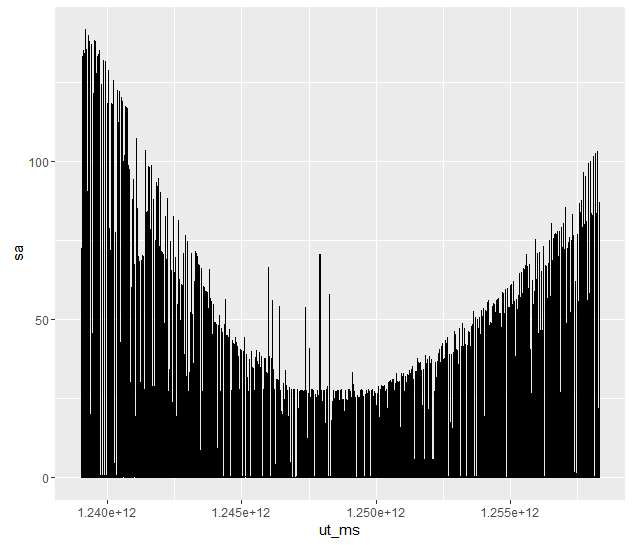
\includegraphics[width=2in]{Assets/saaf1500k850k.png}
\end{center}
\newline \par 
Los datos, sin embargo, presentan varias lagunas y varias etapas con discontinuidades. Se pretende, intuitivamente, buscar alguna relación entre estos datos y los comandos recibidos remotamente para constatar que existe alguna relación. De la misma manera, se espera que exista una relación directa con los distintos eventos como eclipses que puedan haber sucedido.

\end{document}